\documentclass[11pt,a4paper]{article}
\usepackage[utf8]{inputenc}
\usepackage[german]{babel}
\usepackage{amsmath}
\usepackage{amsfonts}
\usepackage{amssymb}
\usepackage{kpfonts}
\usepackage{units}
\usepackage{graphicx}
\usepackage{float}

\usepackage[left=2cm,right=2cm,top=2cm,bottom=2cm]{geometry}


\begin{document}

\pagestyle{empty}

\begin{enumerate}
	
	\item \emph{Halbleiter}
	
	\begin{itemize}
		
		\item 	Struktur der Kristalle $\rightarrow$ Diamantstruktur (rein kovalente Bindung) oder Zinkblende (kovalent-ionische Bindung)
		
		\item Elementhalbleiter (Si, Ge) oder Verbindungshalbleiter (III-V InP GaAs InSb, II-VI ZnS)
		
		\item Grundlegende Beschreibung $\rightarrow$ Bändermodell
		\begin{itemize}
			
			\item an den Atomrumpf gebundene Elektronen, Annäherung der Atome, Überlapp der Wellenfunktionen, Aufspalten der Einzelelektronenniveaus, je mehr Atome desto mehr erlaubte energetisch erlaubte Zustände $\rightarrow$ Bänder
			
			\item Halbleiter hat moderate Bandlücke ($\unit[1 \dots 4]{eV}$), Fermi-Niveau liegt zwischen Valenz- und Leitungsband, für Leitfähigkeit sind Ladungsträger in Leitungsband notwendig, Anregung vom Valenzband durch thermische Anregungen oder Photonen, Stromtransport durch Elektronen und Löcher
			
		\end{itemize} 
			
			\item direkte, indirekte Halbleiter, unterschiedliche Bandstruktur, bei indirekten Halbleitern Anregung ins Leitungsband nur unter Beteiligung von Phononen
		
			\item intrinsischer Halbleiter/extrinsischer Halbleiter jenachdem ob Ladungsträgerdichte durch Halbleiter oder durch Dotierstoff bestimmt wird
			
			\item Dotierung $\rightarrow$ gezieltes Einbringen von Störstellen, Veränderung der elektrischen Leitfähigkeit, Einbringen von Störstellen erzeugt zusätzliche lokale Energieniveaus in der Bandlücke (Akzeptorniveaus nahe der Valenzbandkante durch Akzeptoren, Donatorniveaus nahe Leitungsbandkante durch Donatoren), geringere Energielücke, mehr Elektronen die zum Stromtransport beitragen, Störstellenleitung, Elekronenleitung, Löcherleitung	
		\begin{figure}[H]
			\centering
			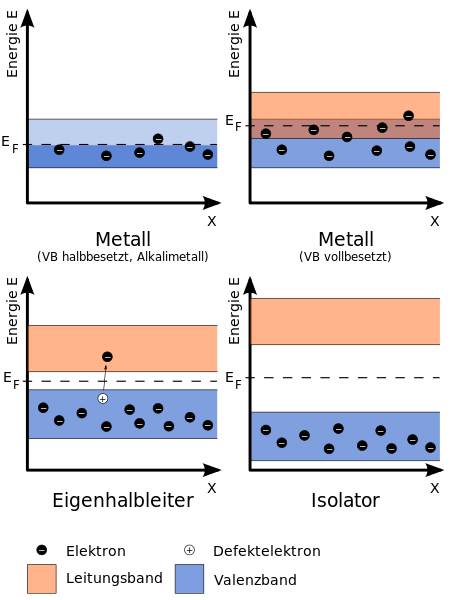
\includegraphics[width=0.3\textwidth]{Energy_band_model.png}
		\end{figure}
					
	\end{itemize}
	
	\item \emph{Halbleiter-Heterostrukturen, Heteroübergänge}
	
	\begin{itemize}
		
		\item typischerweise bei III-V und II-VI Halbleitern
		
		\item Bringt man zwei Halbleiter (verschiedene Bandlücke, verschiedene Dotierung) in Kontakt, so gleichen sich die Ferminiveaus an, es erfolgt eine Bandverbiegung bzw. Diffusion von Ladungsträgern bis die chemischen Potentiale gleich sind, es treten wegen unterschiedlicher Bandlücken auch Banddiskontinuitäten auf, sowie Bandverbiegungen
		\begin{figure}[H]
			\centering
			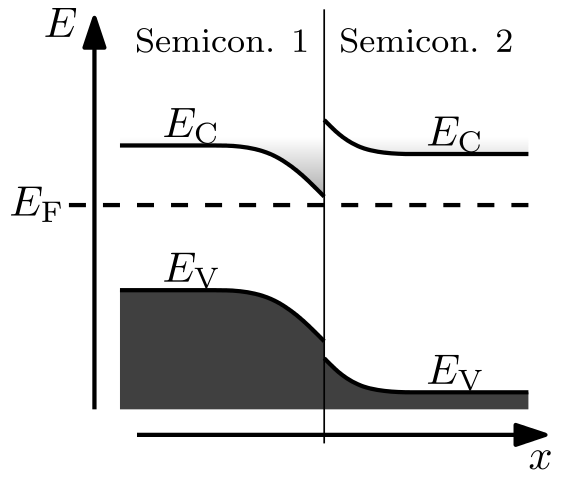
\includegraphics[width=0.3\textwidth]{Straddling_gap_heterojunction_band_diagram.png}
		\end{figure}
		
		\item 
		
	\end{itemize}
	
\end{enumerate}

\end{document}